\section{Technical Information}
\label{sec:Tech}

\subsection{AWS-hosted database}

Figure \ref{fig:er_model} shows the entity relationship model of the project. The information contained in the model is:

\begin{enumerate}

\item Disasters : information of disasters of Colombia from 1998 to 2017, with the following fields: date,  Colombian political division, number of disasters, death, injuries, missing people, families, houses, public and education services infrastructures and some economical  information. (table disasters)
\item Events: name and category of the event (table eventos)
 
\item Political division of Colombia (divipola): ID of division, subdivision and name of both (divipola table)

\item Population estimates: relates population by period, age groups, political division, id, and gender

\item Load tables: temporal tables for loading disasters, political division, population (tables: load\_disasters, load\_divipola, load\_populations)

\item Views: wv\_disasters (summary table for disasters)

\end{enumerate}

The SQL script for the creation of the database on AWS can be download from this link: \\ \url{https://marioceron-case-51.s3.amazonaws.com/final_project/Script_Desastres_DB.sql}{}

 
\begin{figure}[!htb]
\center{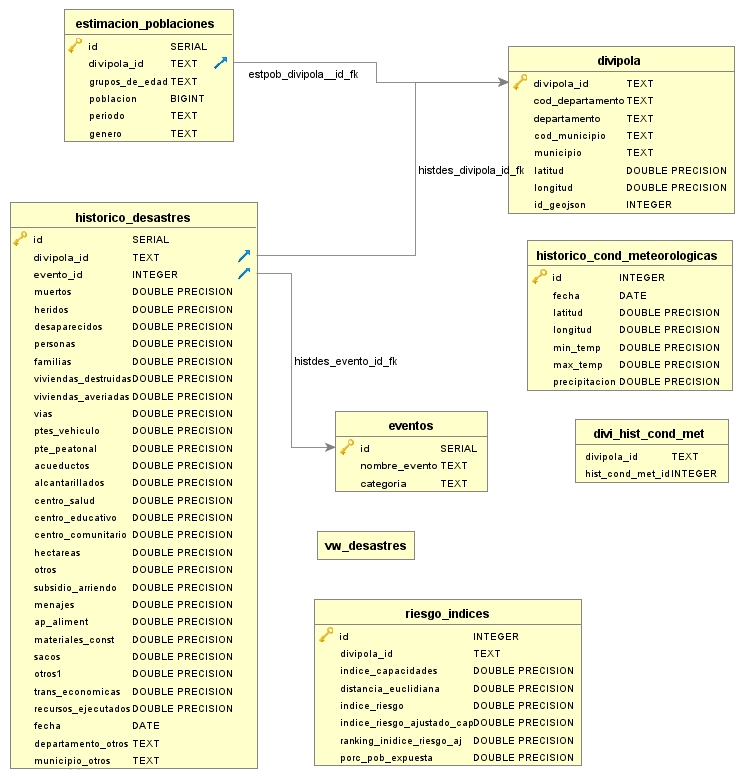
\includegraphics[width=0.95\textwidth]
{Project_Group03_ERModel}}
\caption{Entity relationship model.}
\label{fig:er_model}
\end{figure}

Figure \ref{fig:awsConnection} shows the database uploaded to AWS.

\begin{figure}[!htb]
\center{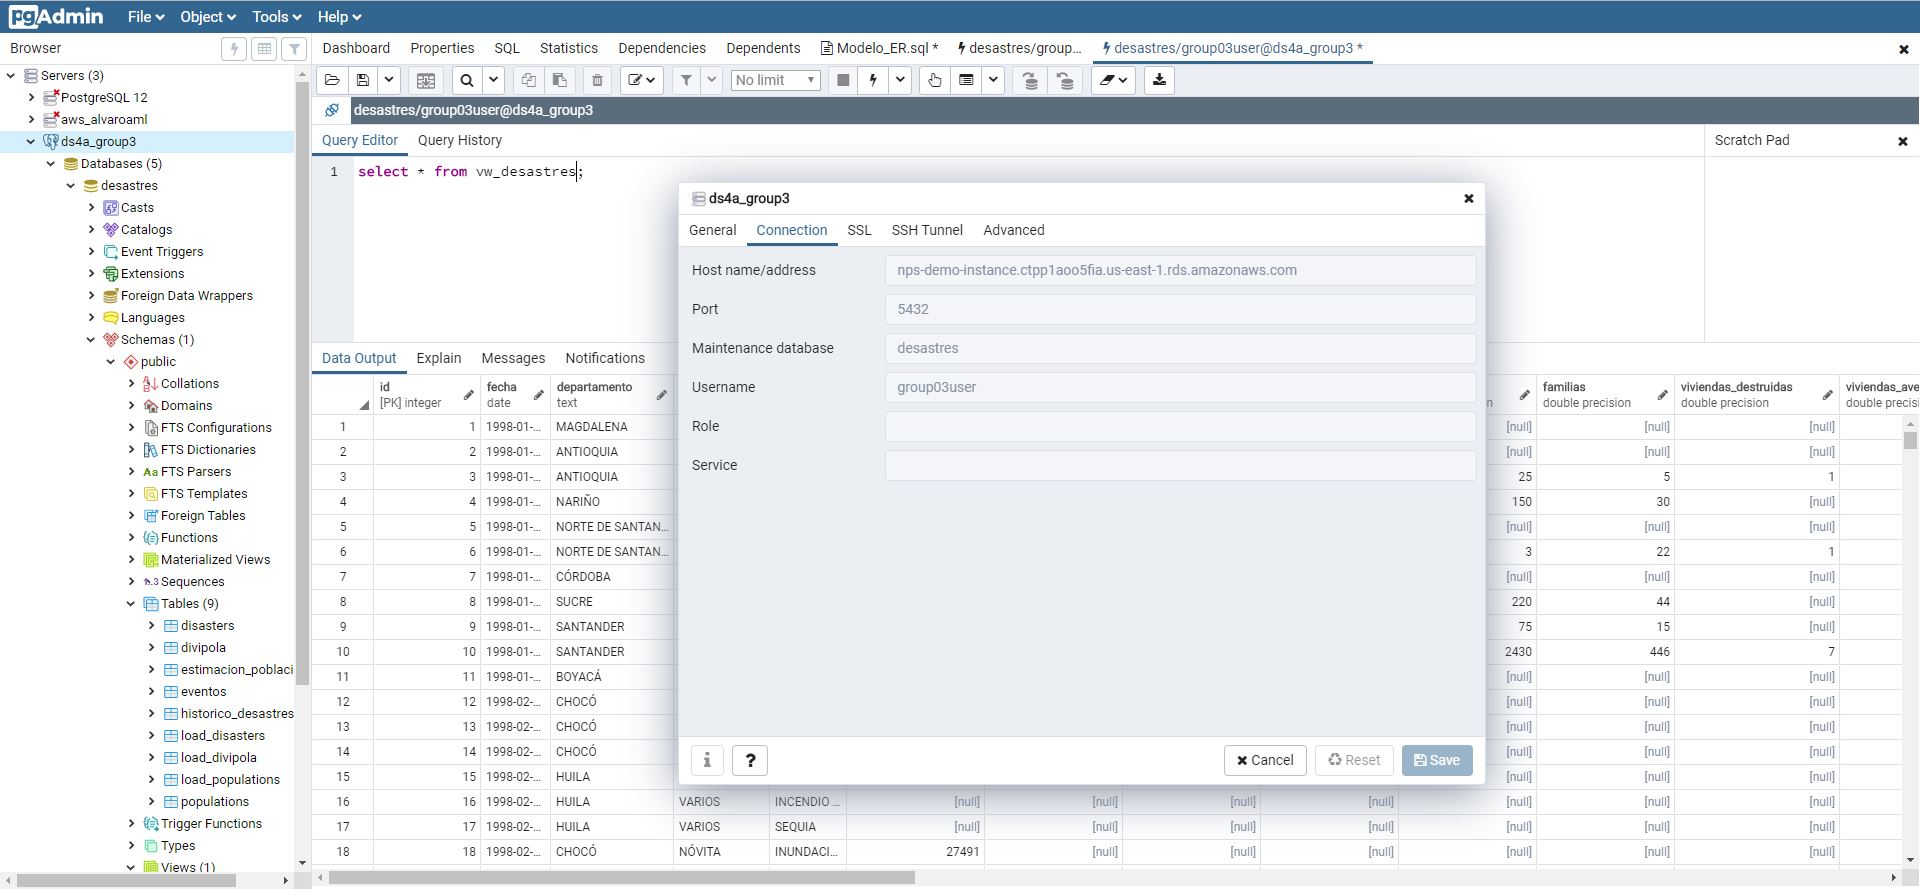
\includegraphics[width=0.95\textwidth]
{Desastres_AWS_Connection}}
\caption{AWS connection.}
\label{fig:awsConnection}
\end{figure}


Figure \ref{fig:databaseLoaded}  shows the database loaded to the AWS hosted database.

\begin{figure}[!htb]
\center{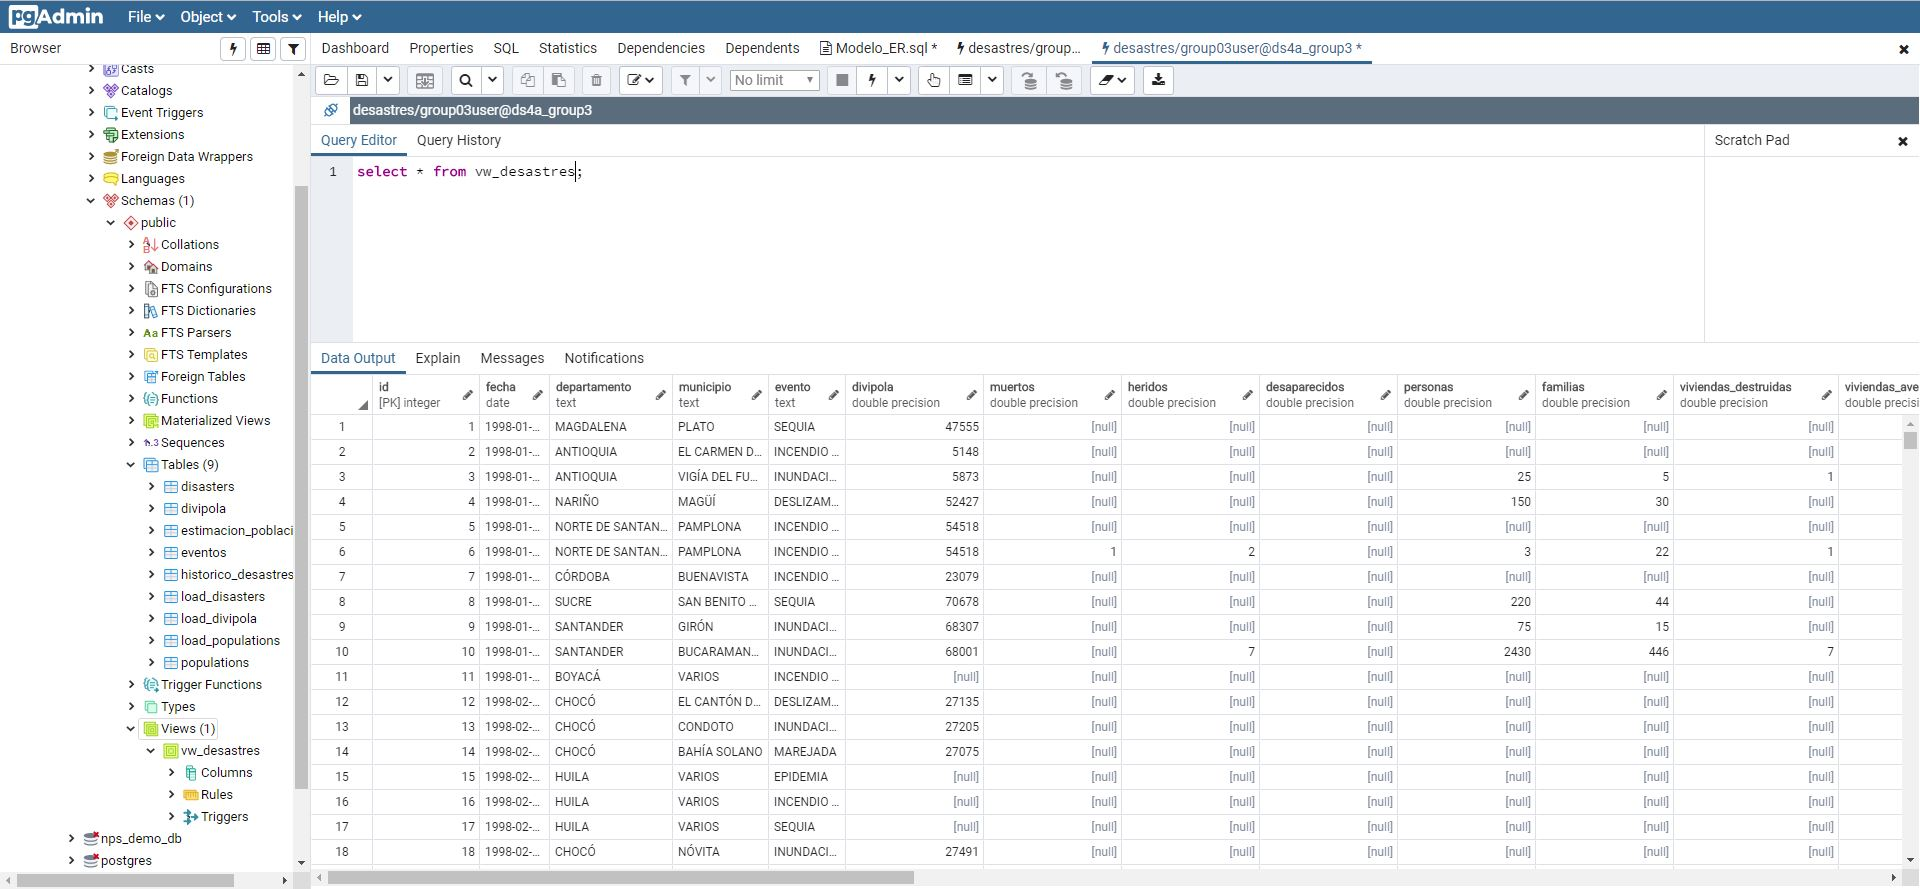
\includegraphics[width=0.95\textwidth]
{Desastres_data}}
\caption{Database loaded to AWS.}
\label{fig:databaseLoaded}
\end{figure}




